\documentclass[11pt,aspectratio=169]{beamer}

\usetheme{Singapore}
\usecolortheme{orchid}

\usepackage[utf8]{inputenc}
\usepackage[russian]{babel}
\usepackage{amsmath}
\usepackage{amsfonts}
\usepackage{amssymb}
\usepackage{graphicx}
\usepackage{bibentry}
\usepackage{wasysym}
\usepackage[most]{tcolorbox}
\usepackage[normalem]{ulem}

\usepackage{hyperref}

\definecolor{info}{RGB}{62, 180, 137}
\definecolor{warn}{RGB}{128, 0, 0}

\author{Николай Анохин}
\title{Нейросетевые рекомендеры}

%\setbeamercovered{transparent} 
%\setbeamertemplate{navigation symbols}{} 
%\logo{} 
%\institute{} 
%\date{} 
%\subject{} 

\begin{document}

{
\setbeamertemplate{headline}{}

\begin{frame}
\titlepage
\end{frame}

%\begin{frame}
%\tableofcontents
%\end{frame}

}

\begin{frame}{Программа модуля}
\begin{tabular}{ l | l | c | c }
{\bf Дата} & {\bf Тема} & {\bf Семинар} & {\bf Домашка} \\
\hline
2021-09-30 & Рекомендательные сервисы в продакшене & \checked &  \\
2021-10-07 & Метрики и базовые подходы & \checked &  \\ 
2021-09-14 & Классические алгоритмы рекомендаций & \checked & \checked  \\
{\color{info} 2021-09-21} & {\color{info} Нейросетевые рекомендеры} & {\color{info} \checked} &  \\
2021-09-28 & Нерешенные проблемы и новые направления & \checked & 
\end{tabular}
\end{frame}

\begin{frame}{Контекст}

\begin{center}
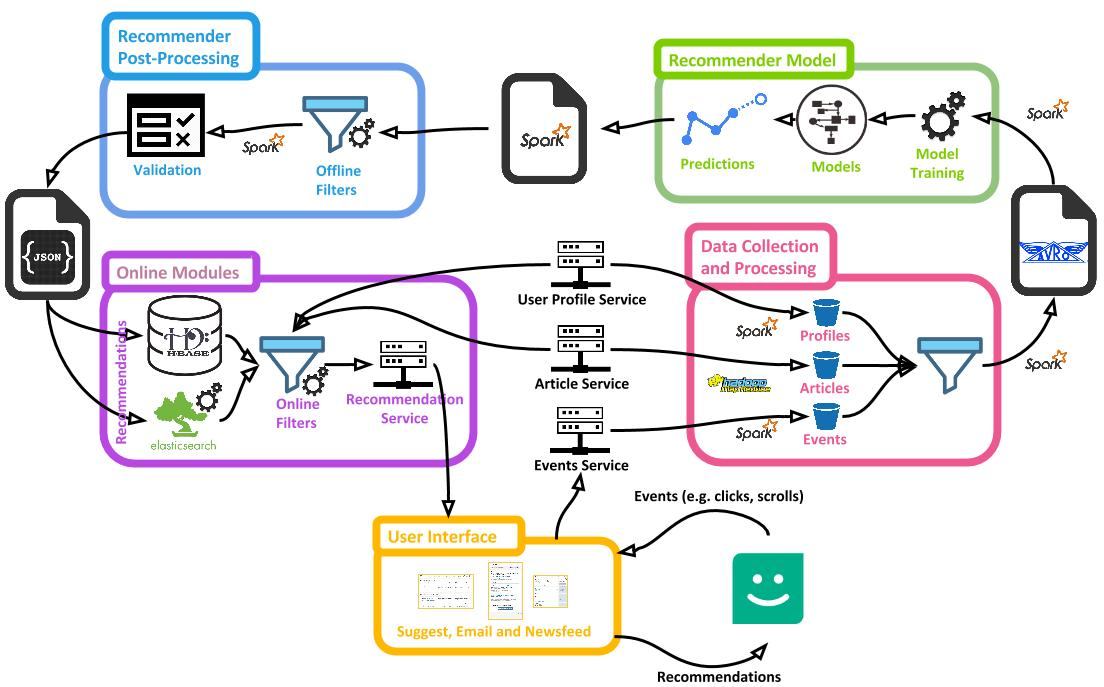
\includegraphics[scale=0.23]{images/mendeley.jpeg}
\end{center}

\end{frame}

\section{От классики к нейросетям}

\begin{frame}{Deep Neural Networks for YouTube Recommendations \cite{YTBE}}

\begin{center}
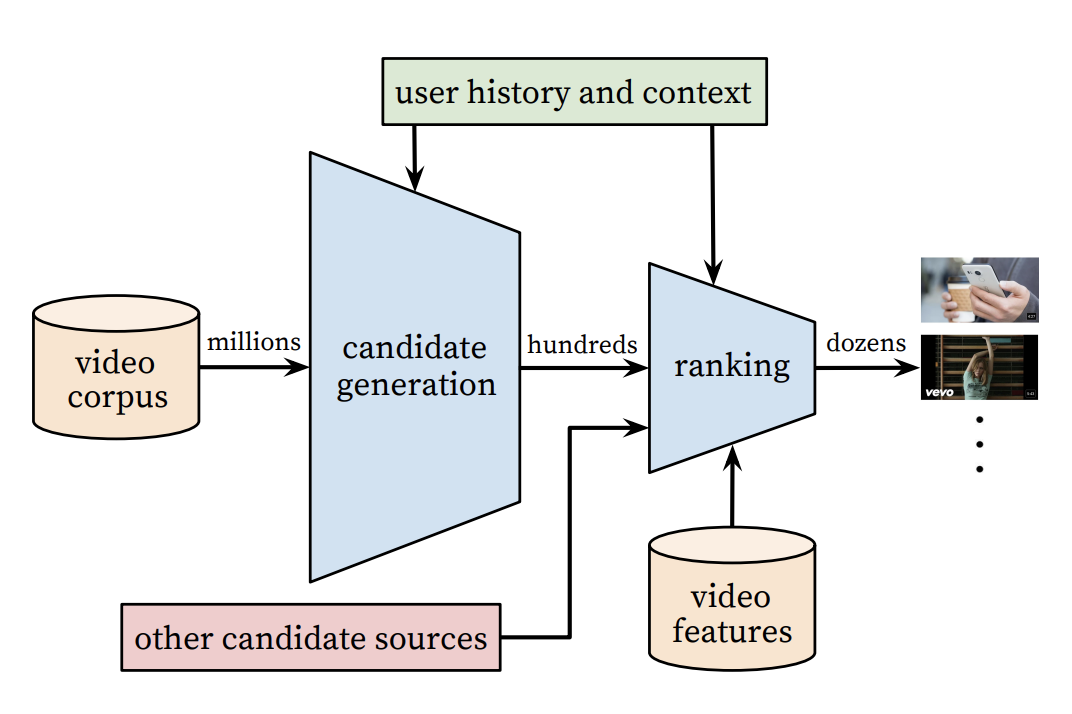
\includegraphics[scale=0.3]{images/youtube-arch.png}
\end{center}

\begin{tabular}{l l}
Интересность & $\star\star\star\star\star$ \\
Полезность & $\star\star\star\star\star$
\end{tabular}

\end{frame}

\begin{frame}

\begin{tcolorbox}[colback=info!5,colframe=info!80,title=SVD++]
\[
\hat r_{ui} = \mu + b_u + b_i + q_i^T \left( p_u + \frac{1}{\sqrt{|N(u)|}} \sum_j y_j \right)
\]
\end{tcolorbox}

\end{frame}

\begin{frame}

\begin{center}
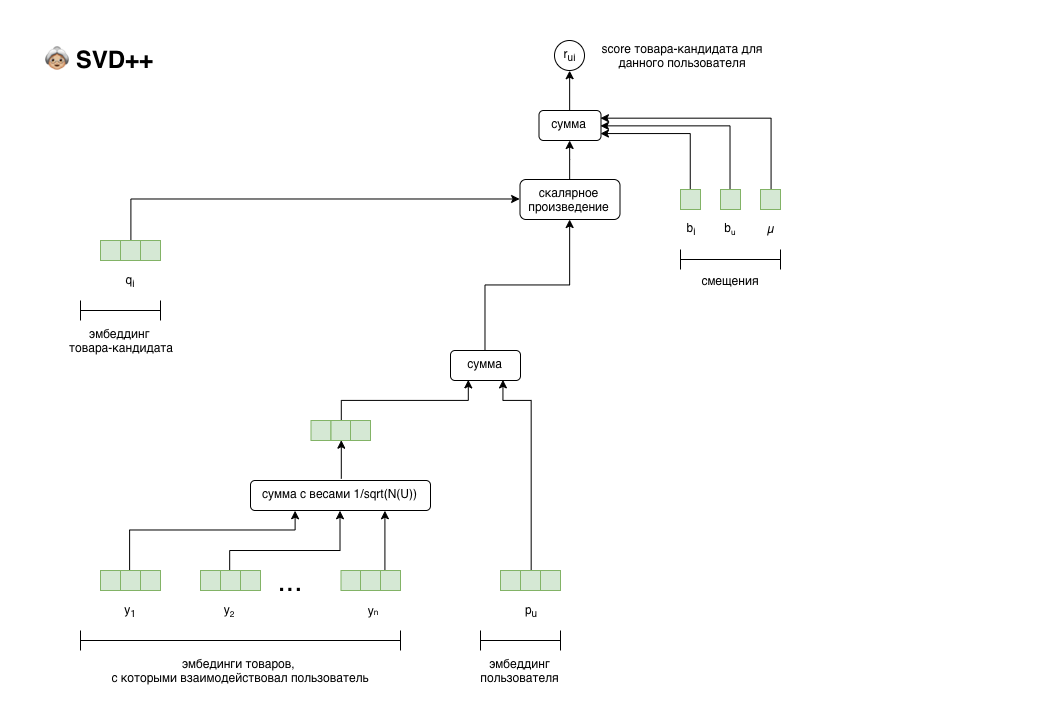
\includegraphics[scale=0.3]{images/svdpp.png}
\end{center}

\end{frame}

\begin{frame}

\begin{center}
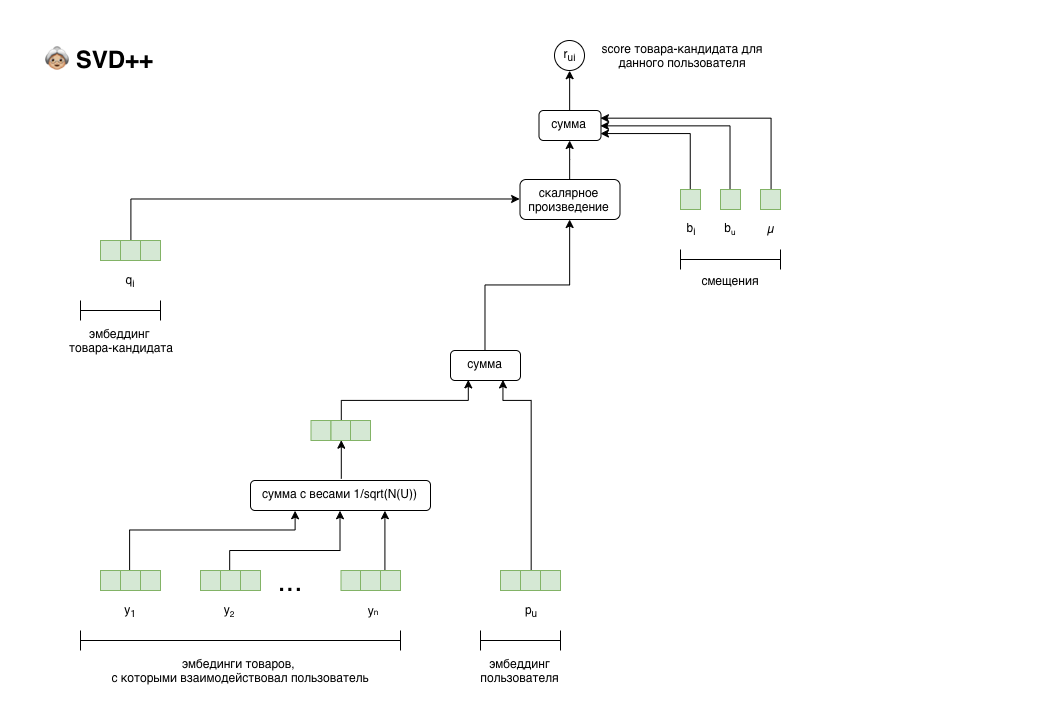
\includegraphics[scale=0.3]{images/svdpp.png}
\end{center}

\end{frame}

\begin{frame}

\begin{center}
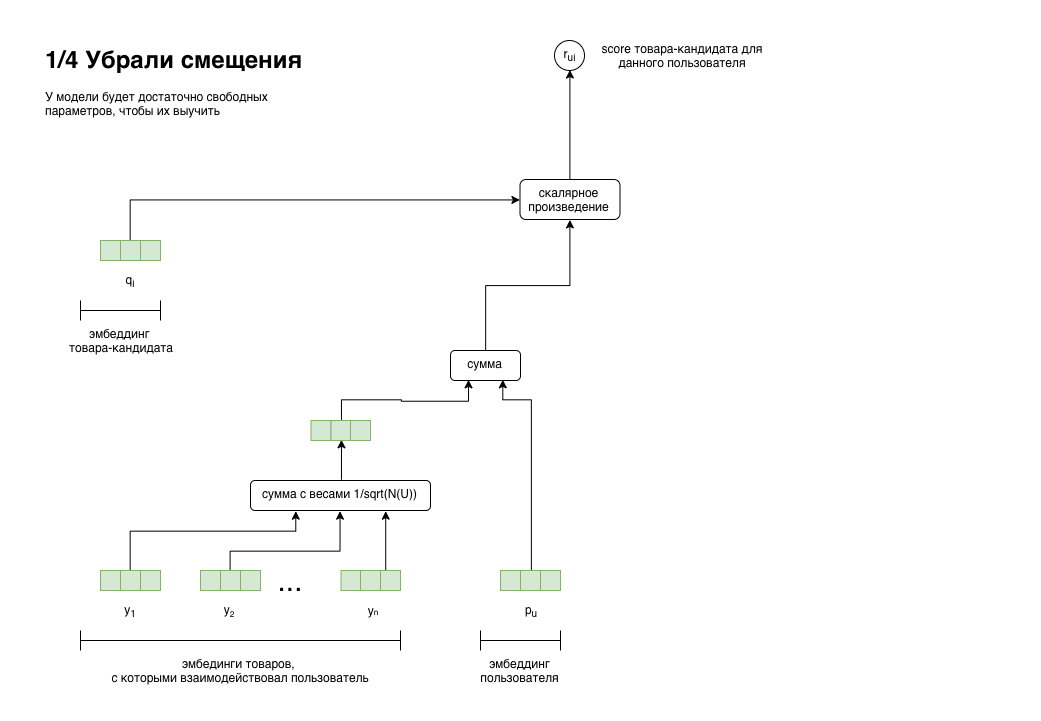
\includegraphics[scale=0.3]{images/svdpp-bias.png}
\end{center}

\end{frame}

\begin{frame}

\begin{center}
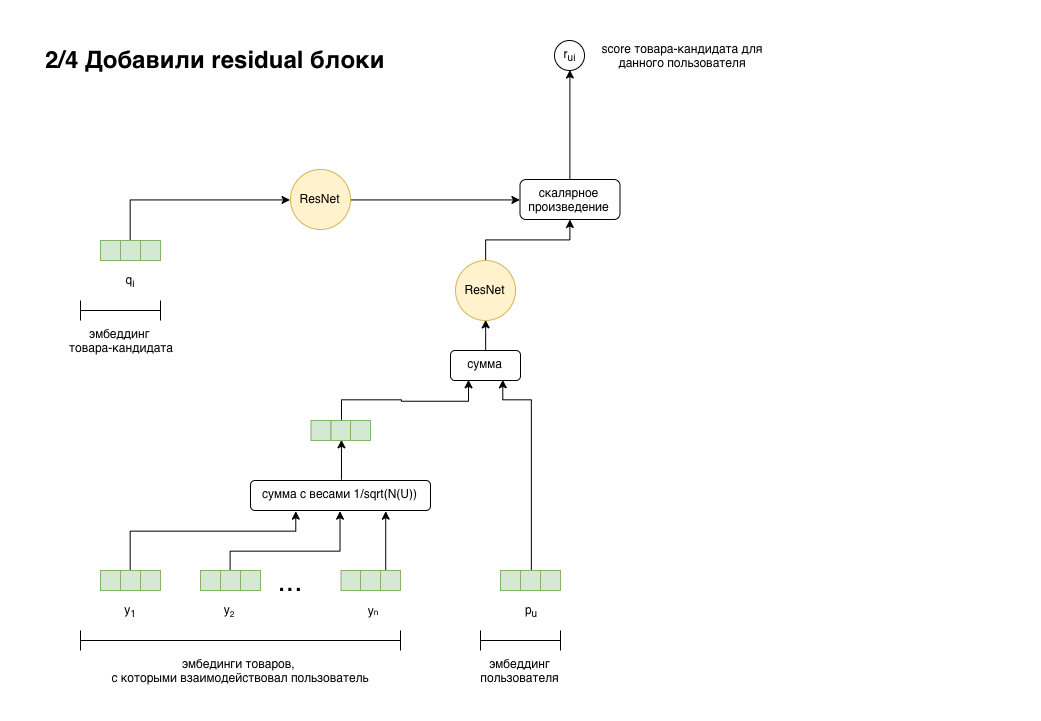
\includegraphics[scale=0.3]{images/svdpp-res.png}
\end{center}

\end{frame}

\begin{frame}

\begin{center}
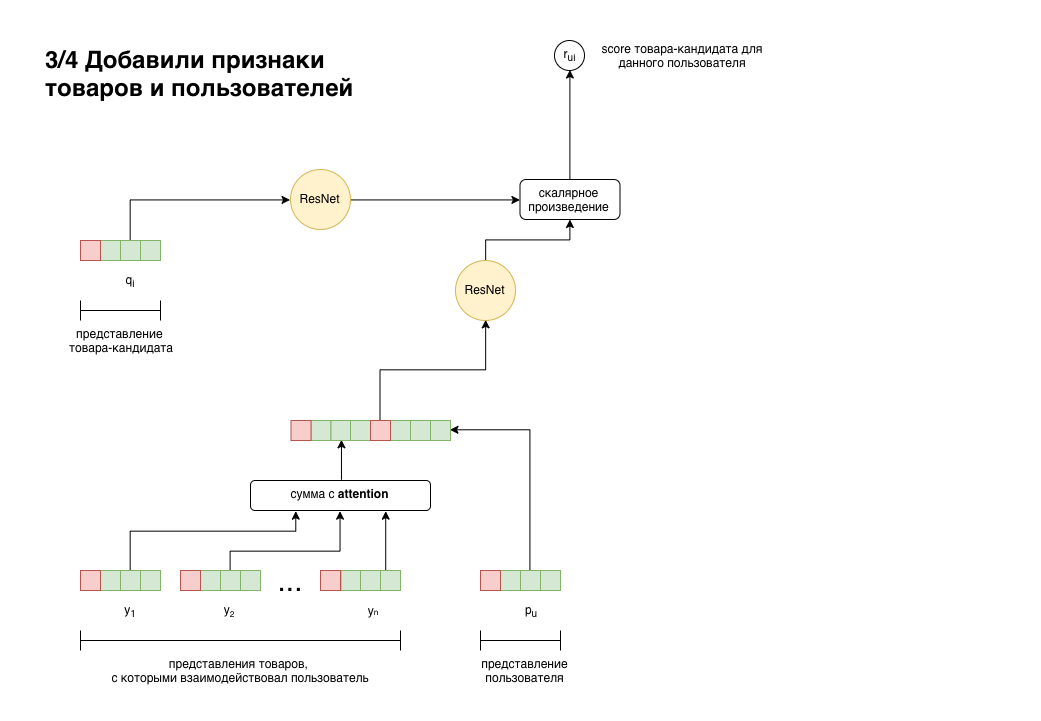
\includegraphics[scale=0.3]{images/svdpp-features.png}
\end{center}

\end{frame}

\begin{frame}

\begin{center}
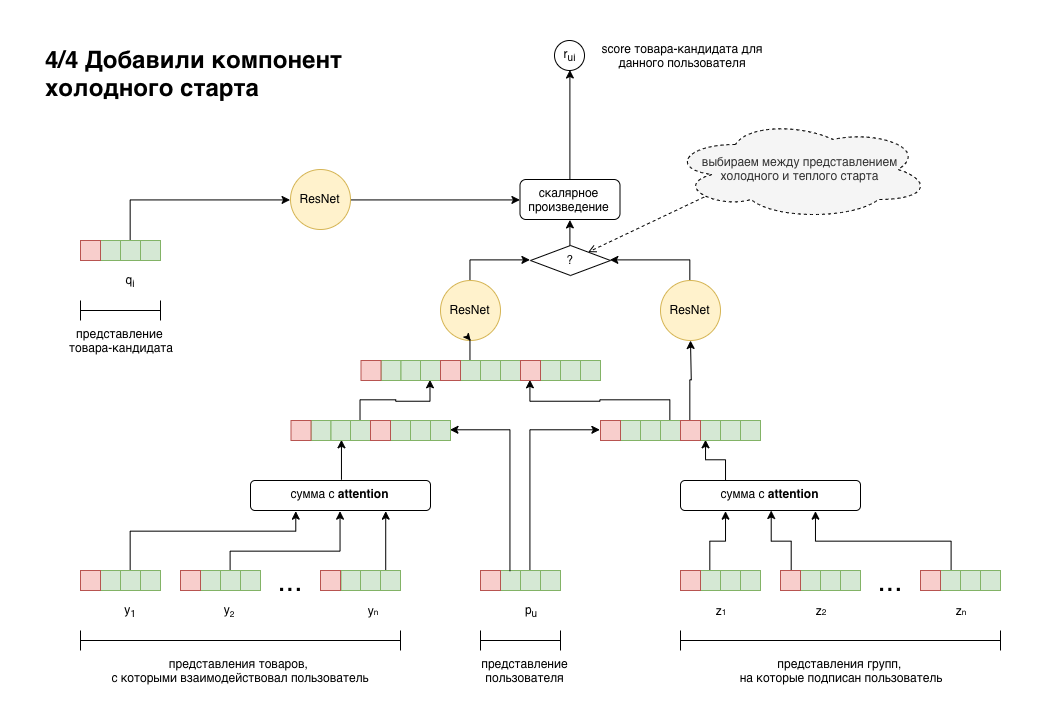
\includegraphics[scale=0.3]{images/svdpp-export.png}
\end{center}

\end{frame}

\section{Истории успеха: отбор кандидатов}

\begin{frame}{Истории успеха: отбор кандидатов}

\begin{tcolorbox}[colback=info!5,colframe=info!80,title=Как оставить след в науке]
\begin{itemize}
\item Изобрести или прикрутить хитрый лосс
\item Изобрести новый метод семплирования данных
\item Заменить скалярное произведение чем-нибудь покруче
\item Заменить эмбединги чем-нибудь покруче
\end{itemize}
\end{tcolorbox}

\end{frame}

\begin{frame}{Neural Collaborative Filtering \cite{NCF}}

\begin{columns}
\begin{column}{0.45\textwidth} 
\begin{center}
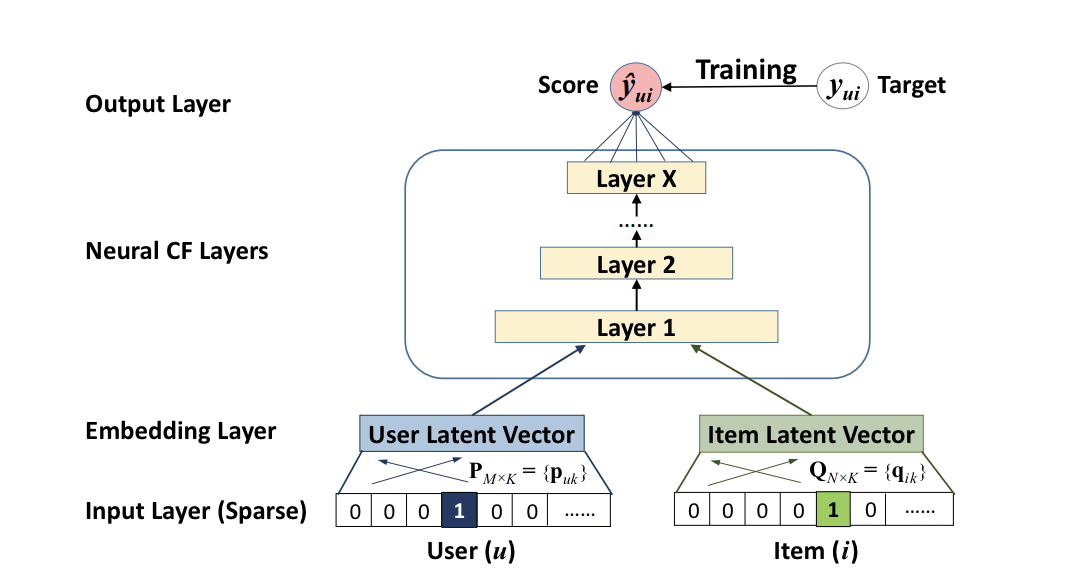
\includegraphics[scale=0.35]{images/ncf.png}
\end{center}
\end{column}
\begin{column}{0.45\textwidth}
\begin{center}
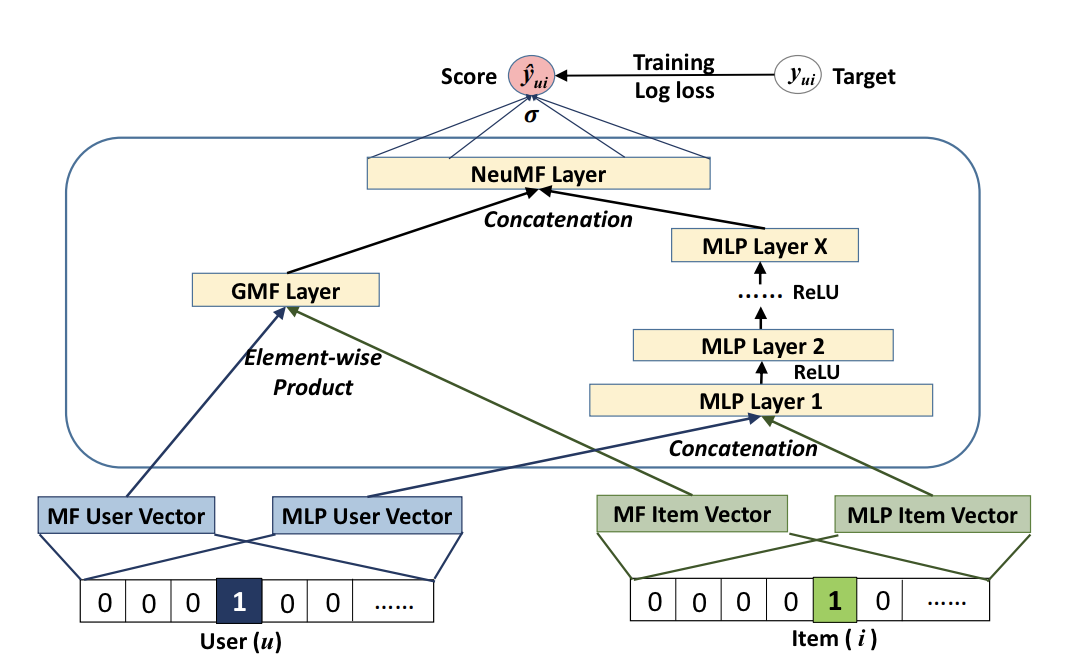
\includegraphics[scale=0.35]{images/nfm.png}
\end{center}
\end{column}
\end{columns}

\begin{tabular}{l l}
Интересность & $\star\star\star$ \\
Полезность & $\star\star\star$
\end{tabular}

\end{frame}

\begin{frame}{Learning Deep Structured Semantic Models for Web Search using Clickthrough Data \cite{DSSM}}

\begin{center}
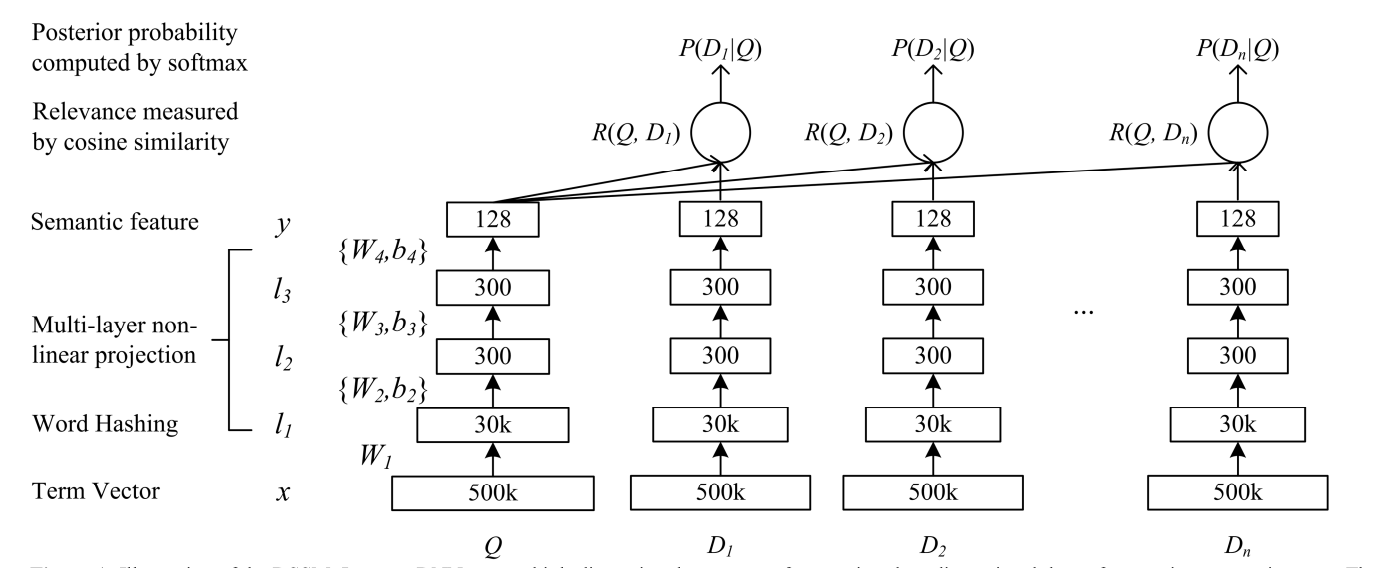
\includegraphics[scale=0.35]{images/dssm.png}
\end{center}

\begin{tabular}{l l}
Интересность & $\star\star\star$ \\
Полезность & $\star\star\star\star$
\end{tabular}

\end{frame}

\begin{frame}{YouTube: отбор кандидатов}

\begin{center}
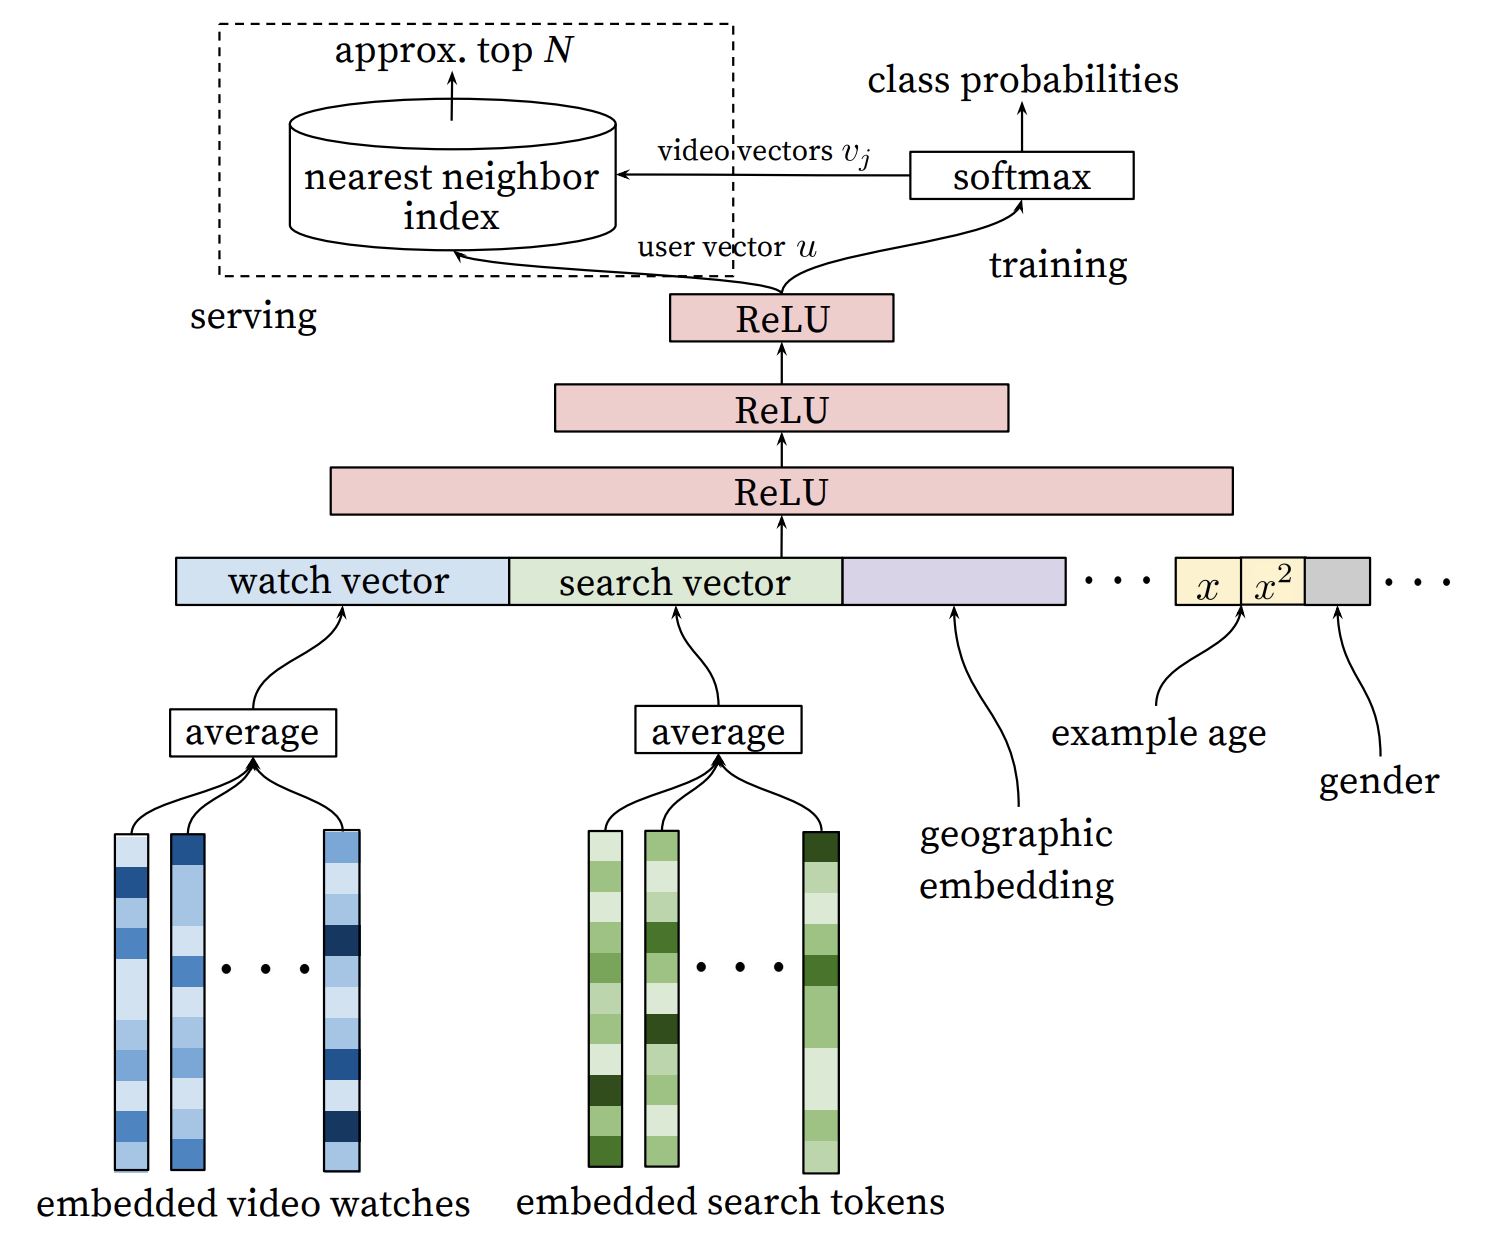
\includegraphics[scale=0.3]{images/youtube-candidate.png}
\end{center}

\end{frame}

\begin{frame}{BERT4Rec: Sequential Recommendation with Bidirectional Encoder Representations from Transformer \cite{BERT4Rec}}

\begin{center}
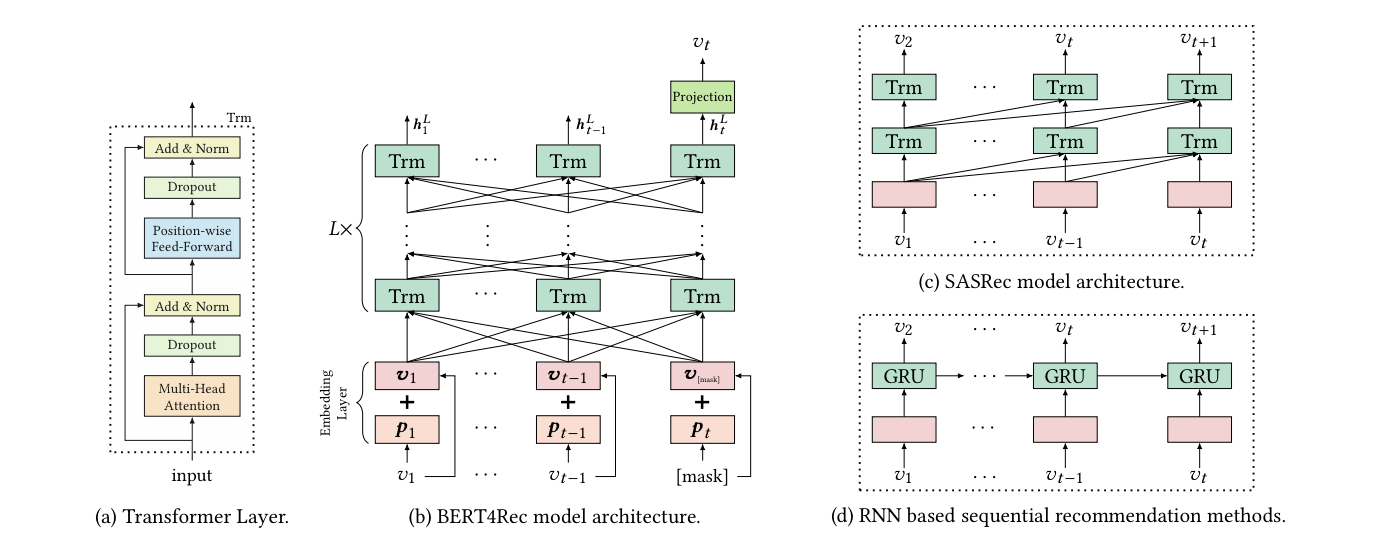
\includegraphics[scale=0.4]{images/bert4rec.png}
\end{center}

\begin{tabular}{l l}
Интересность & $\star\star$ \\
Полезность & $\star$
\end{tabular}

\end{frame}

\begin{frame}{BERT4Rec: эксперименты}

\begin{center}
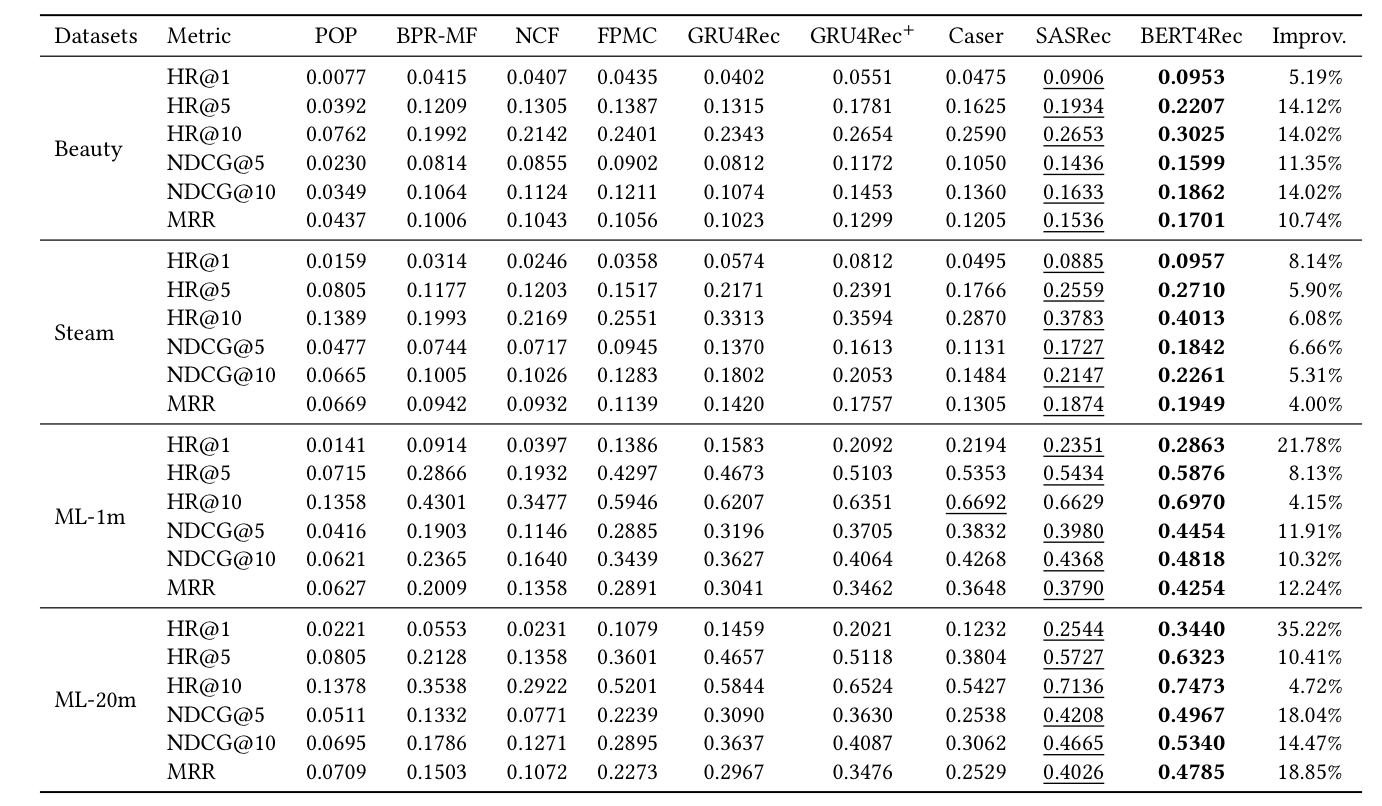
\includegraphics[scale=0.45]{images/bert4rec-table.png}
\end{center}

\end{frame}

\begin{frame}{Deep Feedback Network for Recommendation \cite{DFN}}

\begin{center}
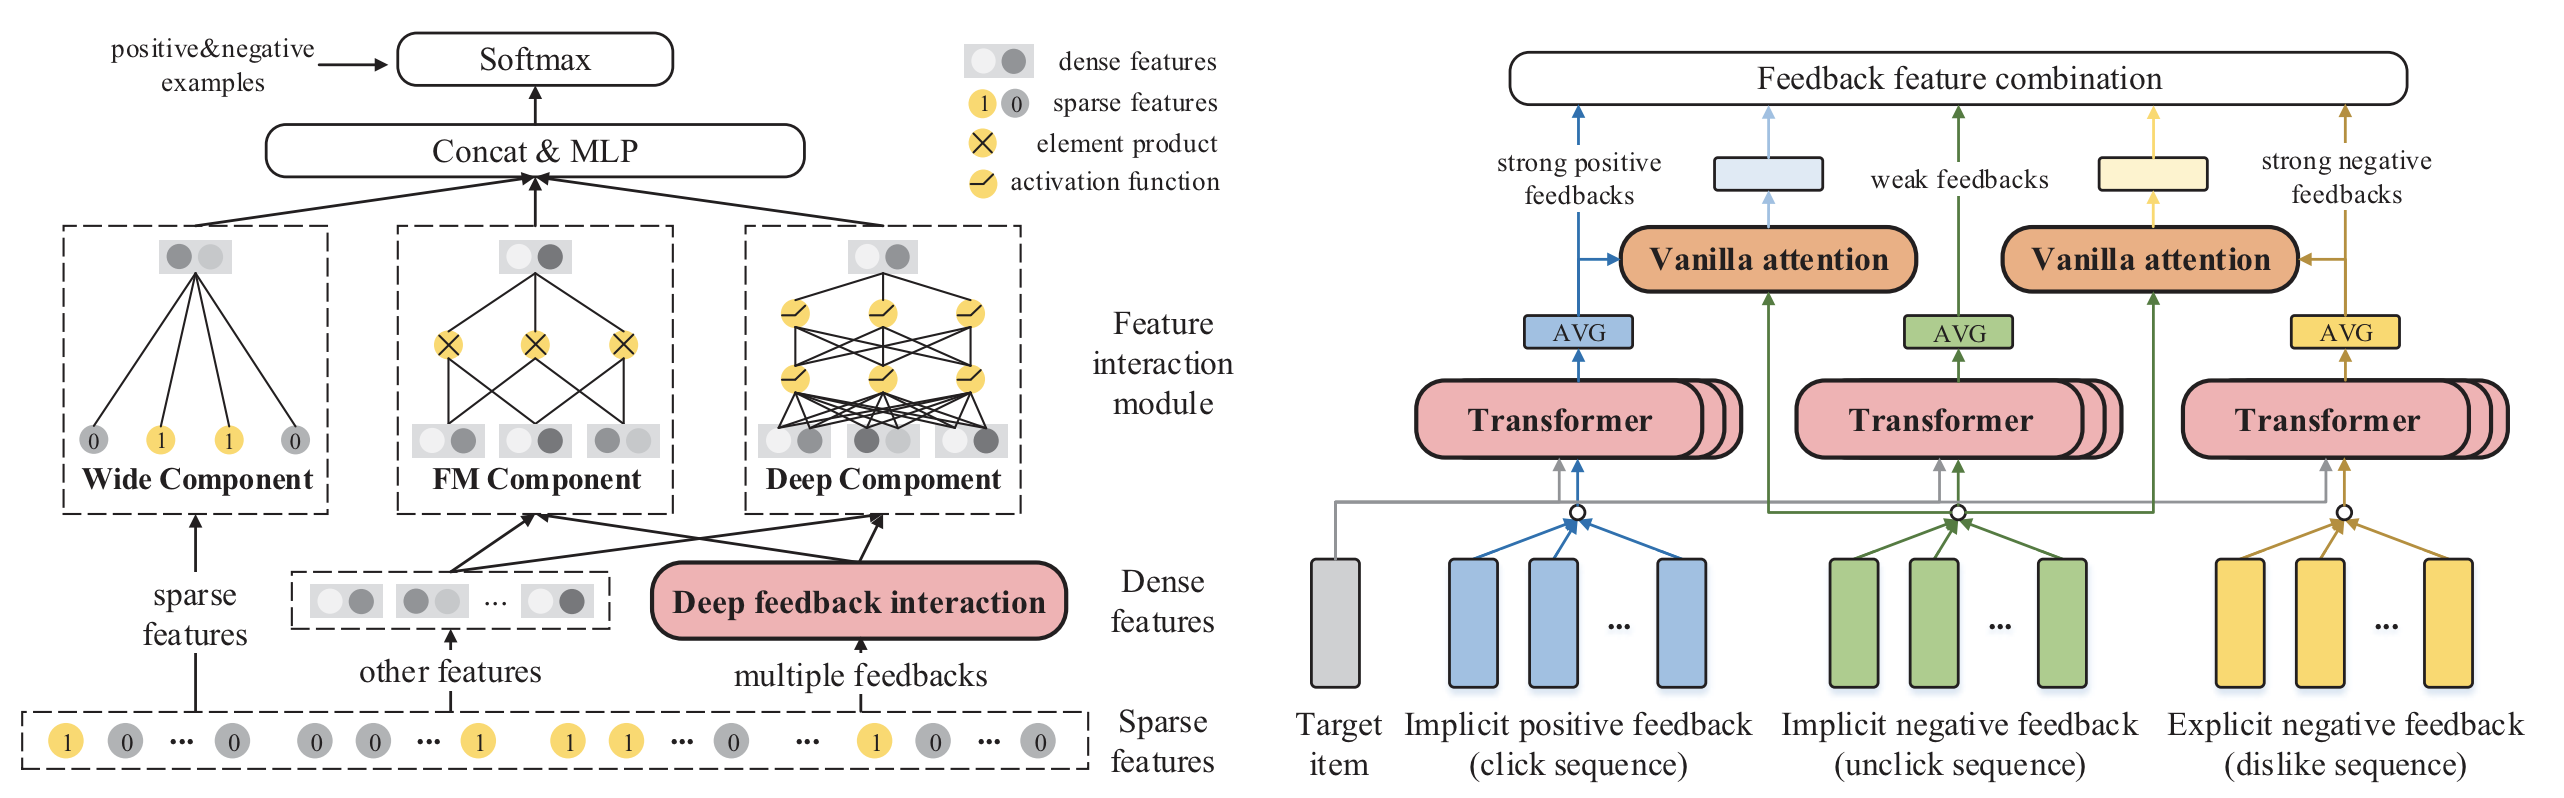
\includegraphics[scale=0.3]{images/dfn.png}
\end{center}

\begin{tabular}{l l}
Интересность & $\star\star\star$ \\
Полезность & $\star$
\end{tabular}

\end{frame}

\begin{frame}{Библиотеки приближенного поиска соседей}
\url{https://github.com/erikbern/ann-benchmarks}

\begin{center}
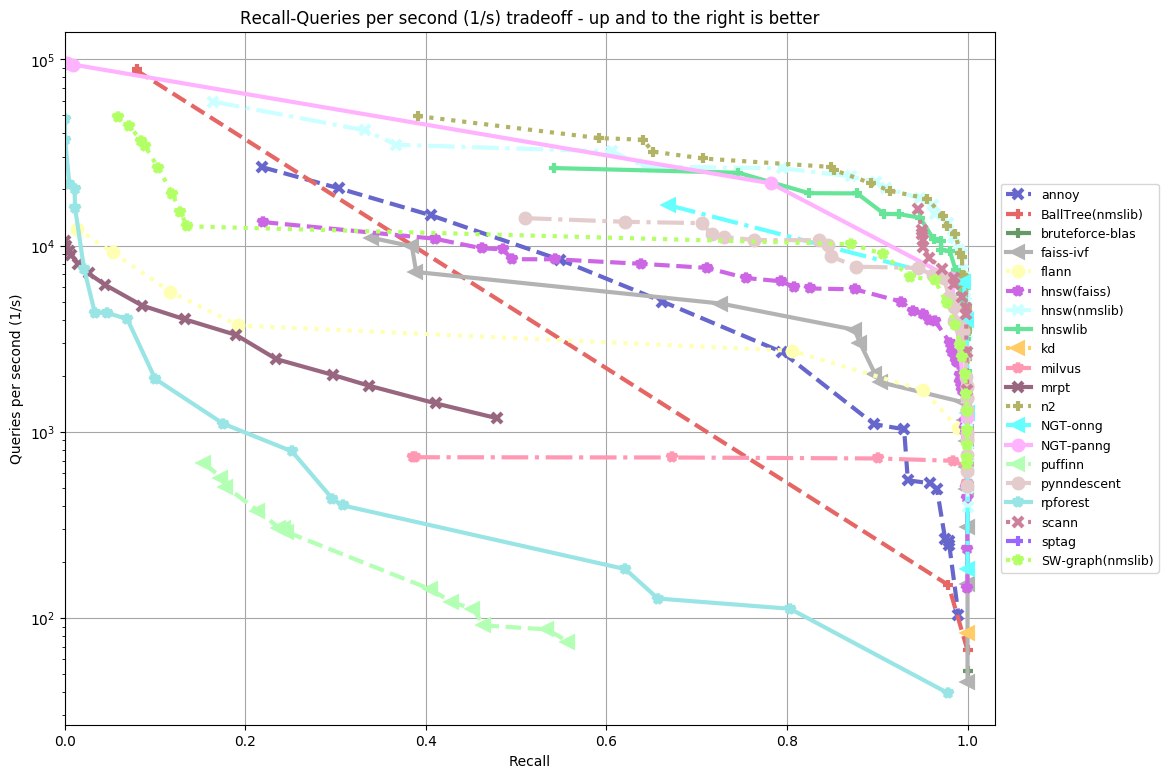
\includegraphics[scale=0.3]{images/ann.png}
\end{center}

\end{frame}

\section{Истории успеха: ранжирование}

\begin{frame}{Истории успеха: ранжирование}

\begin{tcolorbox}[colback=info!5,colframe=info!80,title=Как оставить след в науке]
\begin{itemize}
\item Победить xgboost
\item Пофиксить смещения
\end{itemize}
\end{tcolorbox}

\end{frame}

\begin{frame}{Applying Deep Learning To Airbnb Search \cite{AIRBNB}}

\begin{columns}
\begin{column}{0.45\textwidth} 
\begin{center}
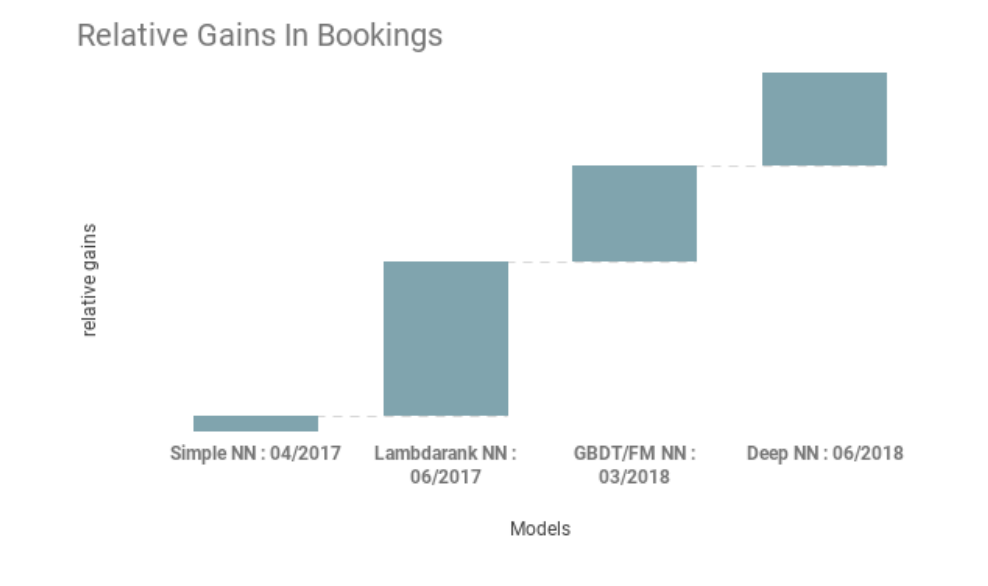
\includegraphics[scale=0.3]{images/airbnb-progression.png}
\end{center}
\end{column}
\begin{column}{0.45\textwidth}
\begin{center}
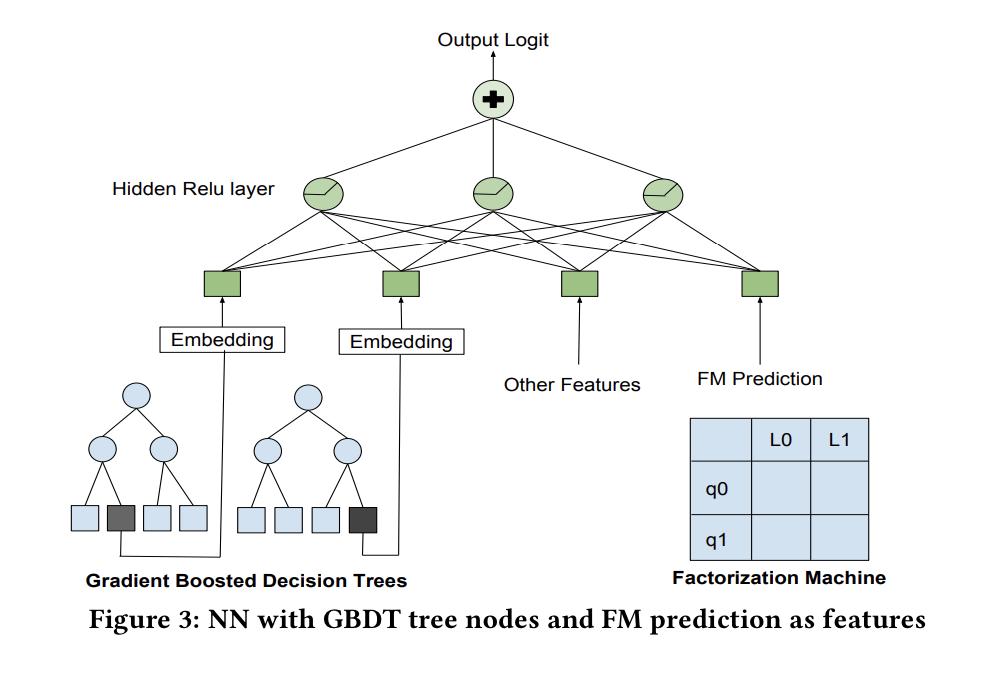
\includegraphics[scale=0.3]{images/airbnb-gbdt.png}
\end{center}
\end{column}
\end{columns}

\begin{tcolorbox}[colback=info!5,colframe=info!80,title=]
...we were able to deprecate all that complexity by simply scaling the training data 10x and moving to a DNN with 2 hidden layers...
\end{tcolorbox}

\begin{tabular}{l l}
Интересность & $\star\star\star\star$ \\
Полезность & $\star\star\star\star\star$
\end{tabular}

\end{frame}

\begin{frame}{YouTube: ранжирование}

\begin{center}
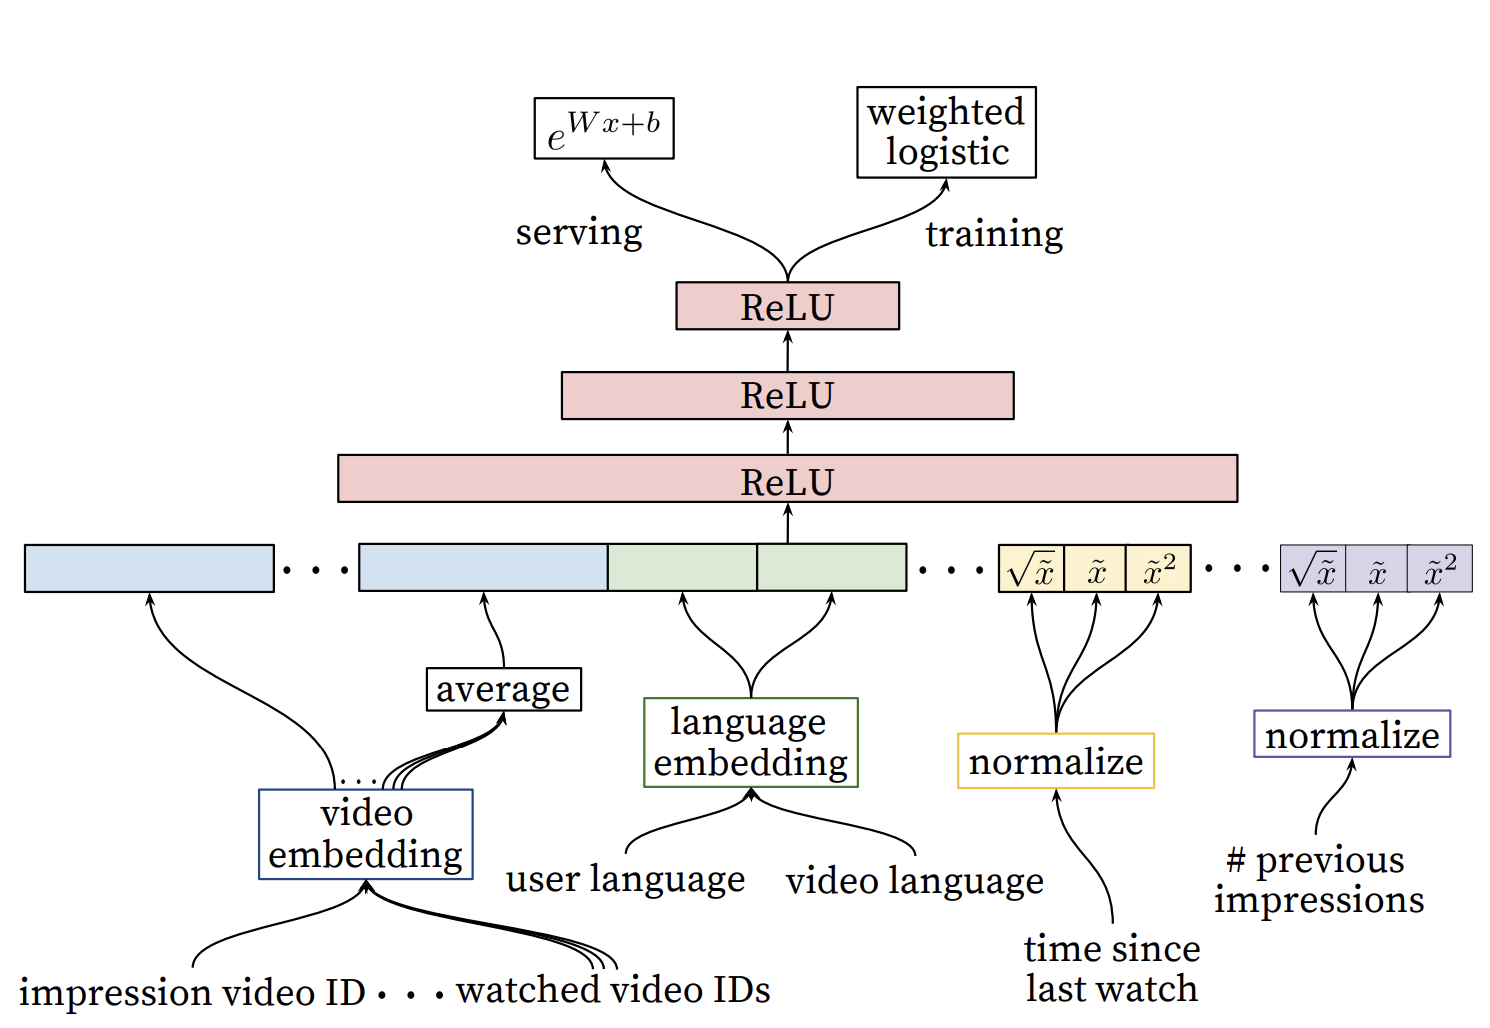
\includegraphics[scale=0.3]{images/youtube-rank.png}
\end{center}

\end{frame}

\begin{frame}{Wide \& Deep Learning: Better Together with TensorFlow \cite{WD}}

\begin{center}
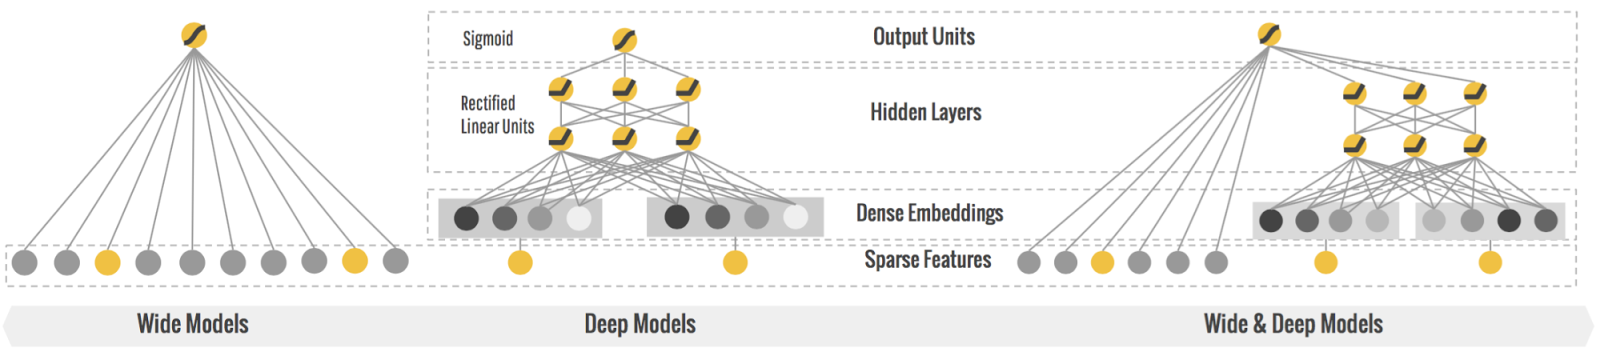
\includegraphics[scale=0.25]{images/widedeep.png}
\end{center}

\begin{tabular}{l l}
Интересность & $\star\star$ \\
Полезность & $\star\star\star\star$
\end{tabular}

\end{frame}

\begin{frame}{DCN V2: Improved Deep \& Cross Network and Practical Lessons for Web-scale Learning to Rank Systems \cite{DCN}}

\begin{columns}
\begin{column}{0.45\textwidth} 
\begin{center}
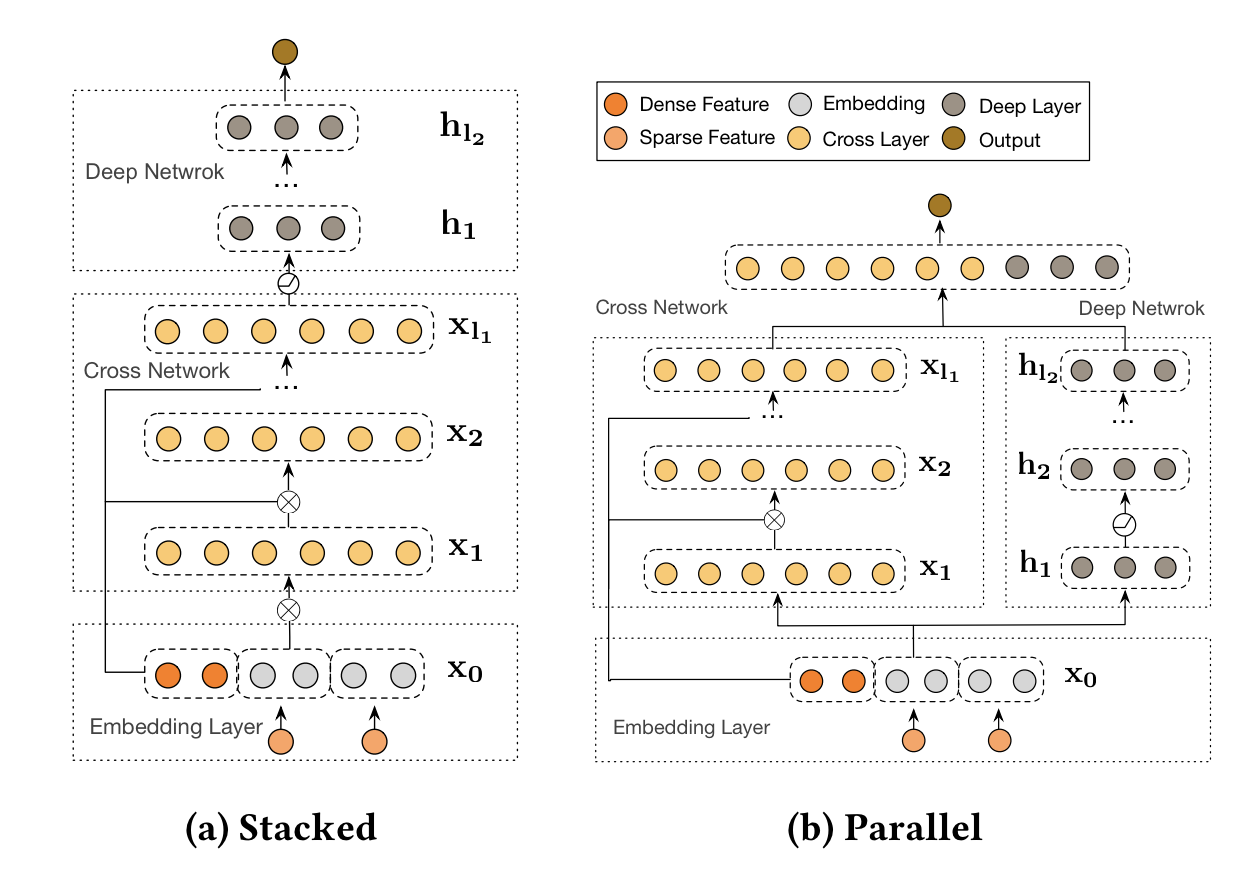
\includegraphics[scale=0.3]{images/dcn-arch.png}
\end{center}
\end{column}
\begin{column}{0.45\textwidth}
\begin{center}
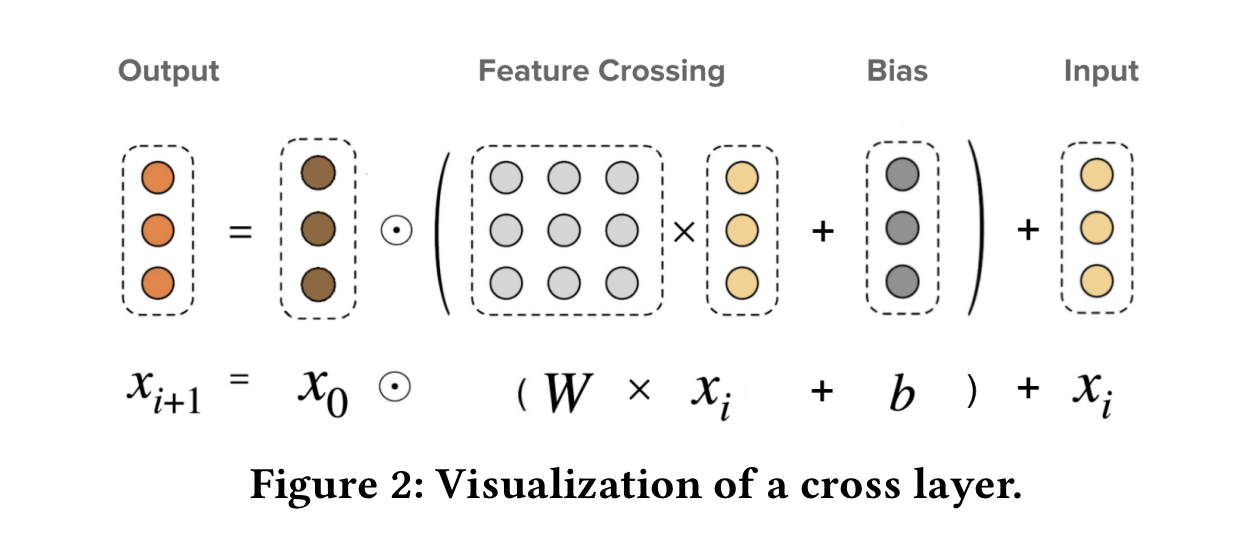
\includegraphics[scale=0.3]{images/dcn-block.png}
\end{center}
\end{column}
\end{columns}

\begin{tabular}{l l}
Интересность & $\star\star\star$ \\
Полезность & $\star\star\star\star$
\end{tabular}

\end{frame}

\begin{frame}{Recommending What Video to Watch Next: A Multitask Ranking System \cite{RANKING}}

\begin{center}
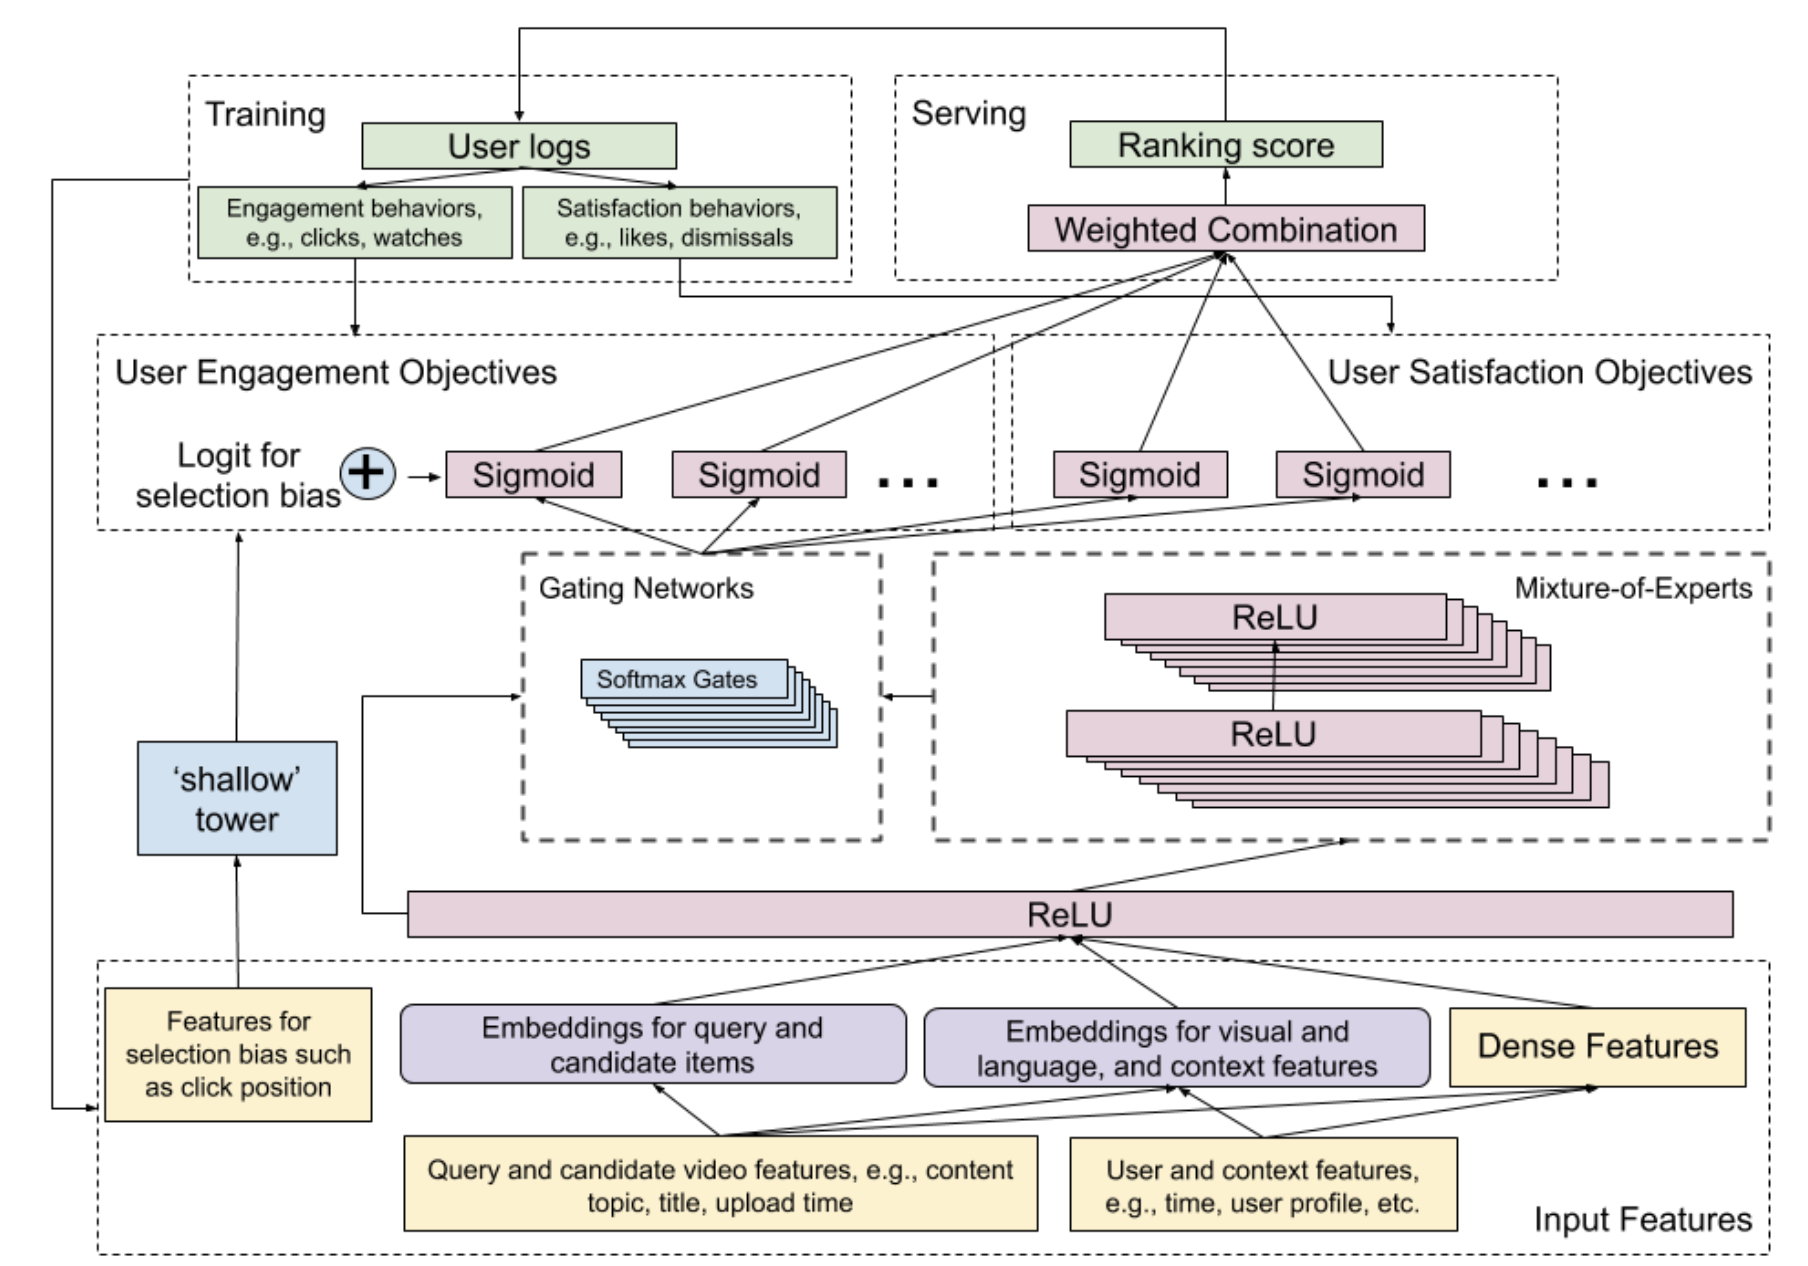
\includegraphics[scale=0.25]{images/multitask.png}
\end{center}

\begin{tabular}{l l}
Интересность & $\star\star\star\star\star$ \\
Полезность & $\star\star$
\end{tabular}

\end{frame}

\section{Истории успеха: контент}

\begin{frame}{Истории успеха: контент}

\begin{tcolorbox}[colback=info!5,colframe=info!80,title=Как оставить след в науке]
\begin{itemize}
\item Решить проблему холодного старта, хитро обучив эмбединги
\end{itemize}
\end{tcolorbox}

\end{frame}

\begin{frame}{PinSage: A new graph convolutional neural network for web-scale recommender systems \cite{PINSAGE}}

\begin{center}
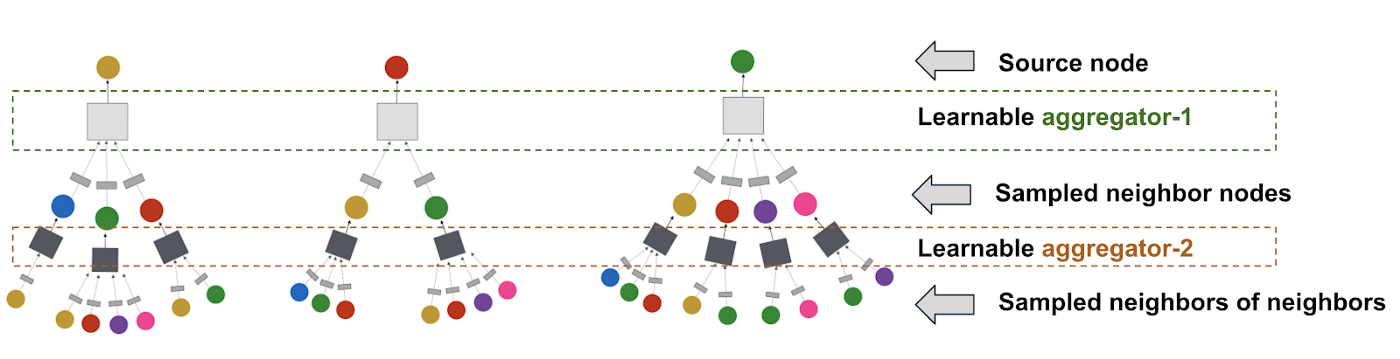
\includegraphics[scale=0.3]{images/pinnersage.png}
\end{center}

\begin{tabular}{l l}
Интересность & $\star\star\star\star\star$ \\
Полезность & $\star\star\star$
\end{tabular}

\end{frame}

\begin{frame}{CB2CF: A Neural Multiview Content-to-Collaborative Filtering Model for Completely Cold Item Recommendations	 \cite{CB2CF}}

\begin{center}
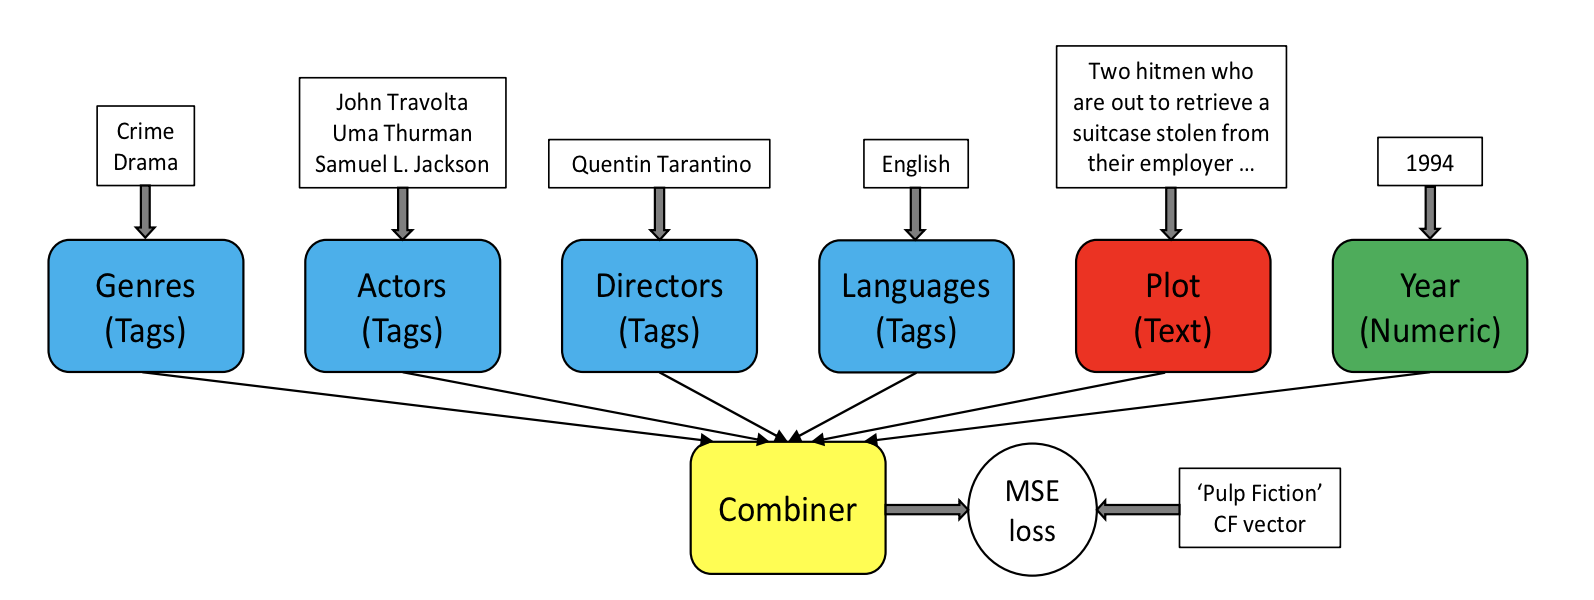
\includegraphics[scale=0.4]{images/cf2cf.png}
\end{center}

\begin{tabular}{l l}
Интересность & $\star\star\star\star$ \\
Полезность & $\star\star\star\star\star$
\end{tabular}

\end{frame}

\section{Итоги}

\begin{frame}{Проблема воспроизводимости \cite{PROGRESS}}

\begin{tcolorbox}[colback=warn!5,colframe=warn!80,title=]
Многие результаты из статей невозможно воспроизвести
\end{tcolorbox}

\begin{tcolorbox}[colback=warn!5,colframe=warn!80,title=]
Некоторые новые алгоритмы работают хуже, чем затюненные бейзлайны
\end{tcolorbox}

\begin{columns}
\begin{column}{0.45\textwidth} 
\begin{tcolorbox}[colback=gray!5,colframe=gray!80,title=]
The CMN method was presented at SIGIR 18 and combines memory networks and neural attention mechanisms with latent factor and neighborhood models
\end{tcolorbox}
\end{column}
\begin{column}{0.45\textwidth}
\begin{center}
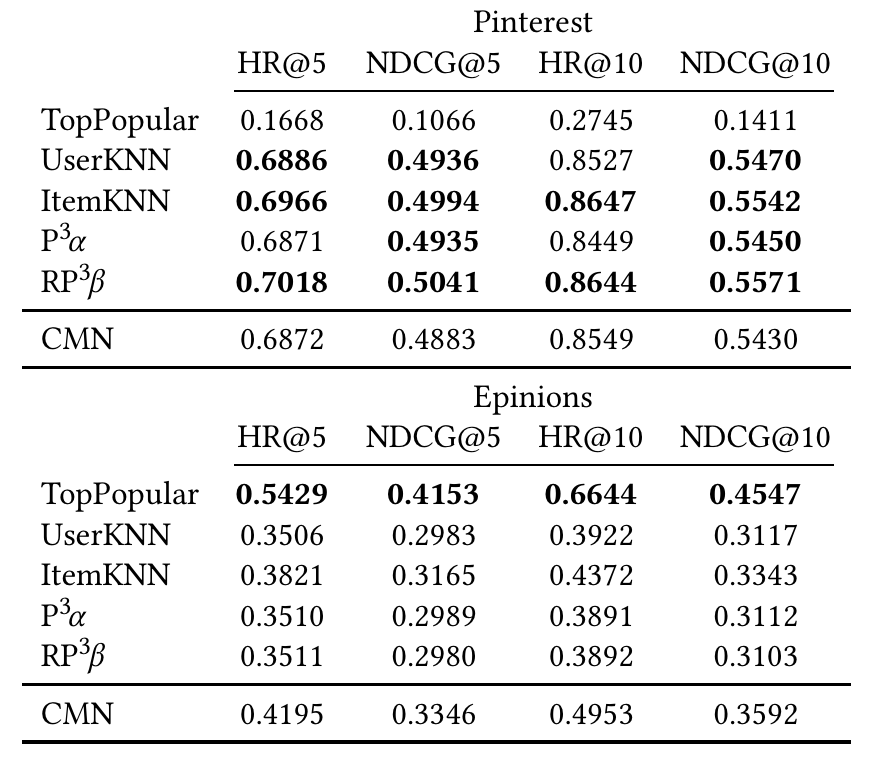
\includegraphics[scale=0.25]{images/progress.png}
\end{center}
\end{column}
\end{columns}

\end{frame}

\begin{frame}{Проблема сравнений \cite{DALMANN}}

\begin{tcolorbox}[colback=warn!5,colframe=warn!80,title=]
Результат сравнения может поменяться на обратный в зависимости от того, по какой метрике сравнивають
\end{tcolorbox}

\begin{center}
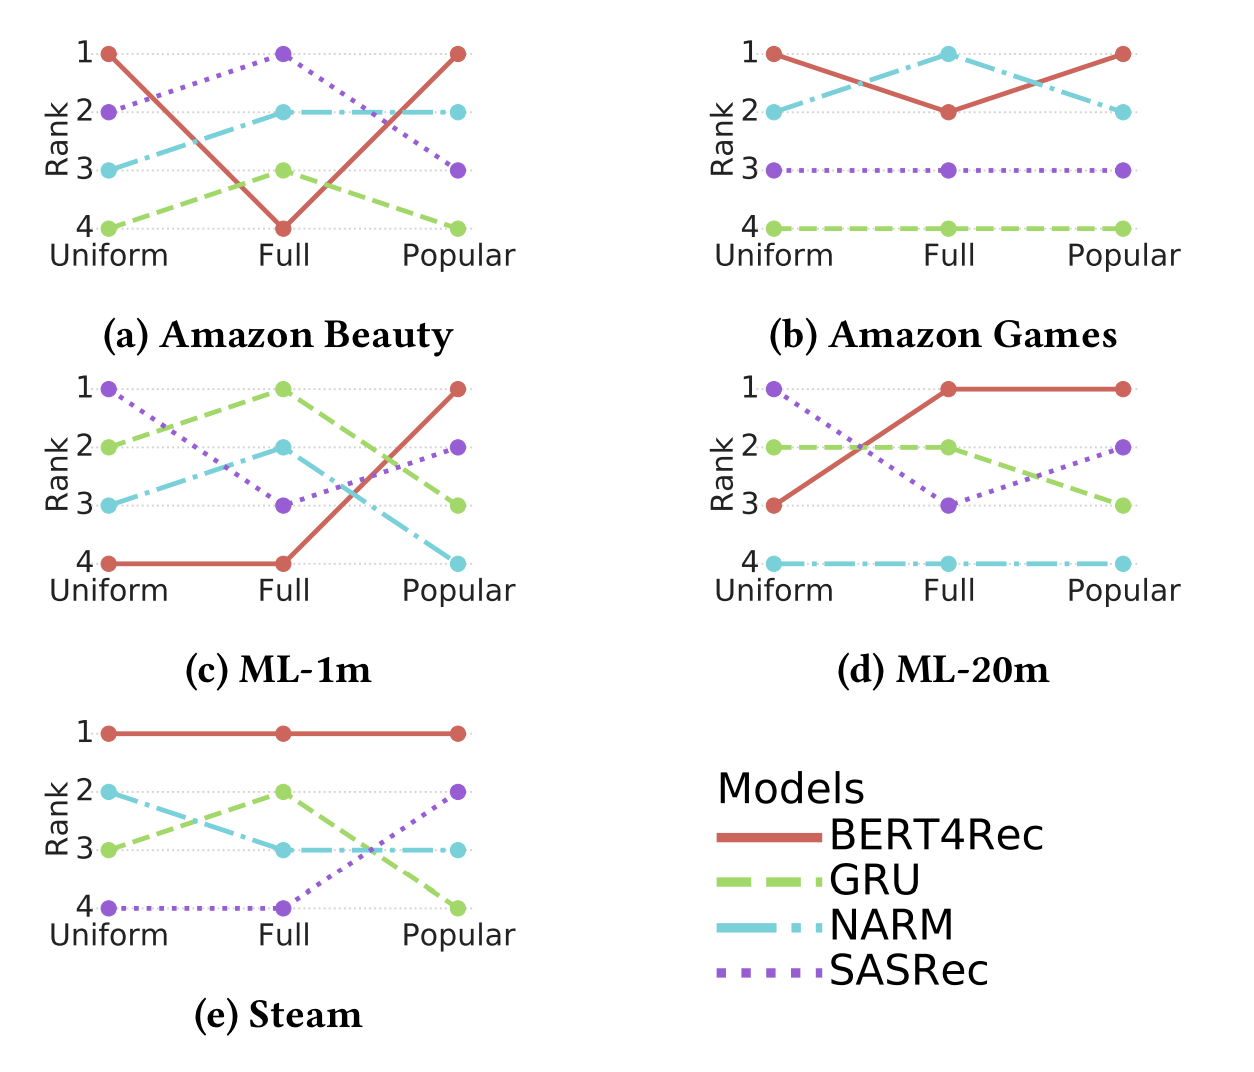
\includegraphics[scale=0.25]{images/compare.png}
\end{center}

\end{frame}

\begin{frame}{Итоги}

\begin{tcolorbox}[colback=info!5,colframe=info!80,title=]
Нейросетевые модели могут заменить любой компонент рекомендательной системы: отборщик кандидатов, ранкер, item2item.
\end{tcolorbox}

\begin{tcolorbox}[colback=info!5,colframe=info!80,title=]
Нейросети помогают добавить inductive bias в рекомендательные модели.
\end{tcolorbox}

\begin{tcolorbox}[colback=warn!5,colframe=warn!80,title=]
Нейросетевой подход не гарантирует выигрыша -- к выбору модели нужно подходить прагматично.
\end{tcolorbox}

\end{frame}

\begin{frame}[allowframebreaks]{Литература}

\bibliographystyle{amsalpha}
\bibliography{references.bib}

\end{frame}

\end{document}
